The manufacturing sector is increasingly driven by the need for efficiency, precision, and cost reduction. Traditional metal fabrication processes, such as the bending of metal sheets, often rely heavily on manual labor. This reliance not only limits production scalability but also introduces variability in product quality and exposes workers to physical strain and repetitive motion injuries. As the industry advances, there is a significant push towards automation to address these challenges and enhance overall productivity.

Robotic automation in manufacturing has emerged as a viable solution to improve process efficiency, ensure consistent product quality, and reduce human labor requirements. The advent of sophisticated robotic systems, such as the Kassow robot, combined with advancements in computer vision and control systems, provides new opportunities to automate complex tasks like metal sheet bending.

The manufacturing sector is driven by the need of increased productivity. The need
for efficiency, precision, safety and cost reduction has led to significant push towards
automation. The industrial growth is currently pushed by the Industrial 4.0: a fourth wave
of technological advancements that is connecting sensors, machines, and other
IT systems. These connected systems, also known as cyberphysical systems, may communicate with one 
another via common Internet-based protocols and use data analysis to self-configure, anticipate 
failure, and react to changes. Industry 4.0 is making it possible to have
flexibility in production by enabling faster and efficient processes. 
High quality.

\begin{figure}[h]
    \centering
    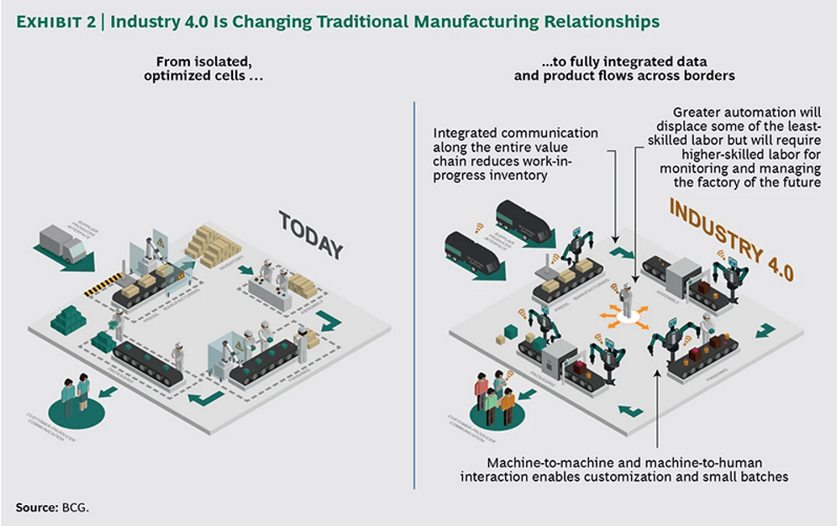
\includegraphics[width=0.75\textwidth]{1. Introduction/1.1 Background/exhibit2.png}
    \caption{Industry 4.0 is changing traditional manufacturing relationships (Source: \cite{russmann2015industry})}
    \label{fig:background-exhibit-2}
\end{figure}


The report by Russmann \cite{russmann2015industry} discusses about the nine pillars
of technological advancements, namely big data and analytics, autonomous robots, simulation,
horizontal and vertical system integration, the industrial internet of things,
cybersecurity, the cloud, additive manufacturing, augmented reality.